\documentclass[10pt,a4paper]{article}
\usepackage[T1]{fontenc}
\usepackage{lmodern,microtype,amsmath,amssymb,mathtools,booktabs,tabularx,array,enumitem,tikz,fancyhdr,xcolor}
\usepackage[margin=21mm,top=19mm,bottom=20mm]{geometry}
\usepackage[colorlinks=true,urlcolor=teal!65!black,linkcolor=teal!65!black]{hyperref}
\hypersetup{pdftitle={The common web and its individual coefficients},pdfauthor={Tom Goertzen, Abel Lacabanne, Daniel Tubbenhauer and Pedro Vaz},pdfsubject={Comparison of arXiv:2611.09114v1 and arXiv:2611.11677v1},citecolor=teal!65!black}
\definecolor{navy}{HTML}{193E50}
\usepackage{titlesec}
\titleformat{\section}{\Large\bfseries\color{navy}}{\thesection}{0.6em}{}
\titleformat{\subsection}{\normalsize\bfseries\color{navy}}{}{0pt}{}
\titlespacing*{\section}{0pt}{.7ex}{1.1ex}
\titlespacing*{\subsection}{0pt}{1.2ex}{.35ex}
\setlength\parindent{0pt}\setlength\parskip{.48em}
\setlist{nosep,leftmargin=*}
\setlength{\headheight}{13pt}
\pagestyle{fancy}\fancyhf{}\fancyhead[L]{\small Guralnick's conjecture}\fancyhead[R]{\small Web and parabolic constructions}\fancyfoot[R]{\small\thepage}\renewcommand\headrulewidth{.2pt}
\newcommand{\C}{\mathbf C}
\newcommand{\R}{\mathcal R_m}
\newcommand{\BS}{\mathcal{BS}}
\newcommand{\CBS}{\mathcal{CBS}}
\newcommand{\ZZ}{\mathbb Z}
\newcommand{\FF}{\mathbb F}
\newtheorem{remark}{Remark}
\newcommand{\eps}{\varepsilon}
\newcommand{\Aword}{\mathsf A}
\newcommand{\Bword}{\mathsf B}
\newcommand{\Cword}{\mathsf C}
\newcommand{\ord}{\operatorname{ord}_v}
\newcommand{\gb}[2]{\genfrac{[}{]}{0pt}{}{#1}{#2}}
\newcolumntype{Y}{>{\raggedright\arraybackslash}X}
\renewcommand{\arraystretch}{1.12}
\begin{document}
{\small AI-assisted comparison note}\par
{\LARGE\bfseries\color{navy} The common web and its individual coefficients}\par
{\large Tom Goertzen, Abel Lacabanne, Daniel Tubbenhauer and Pedro Vaz}
\section*{Overview}
We used an annular web to disprove Guralnick's conjecture on first cohomology for finite simple groups. Independently, Bowman, de la Fuente, Libedinsky and Plaza proved unboundedness in every fixed positive cohomological degree using a product of parabolic symmetrizers. We explain how their construction meets ours in degree one. Both lead to ordinary affine Kazhdan--Lusztig coefficients with the same lower endpoint.

In type~A, singular Bott--Samelson characters and the corresponding split and merge webs describe the same normalized maps in the affine Schur category. Appending two normalized parabolic symmetrizers to their uncorrected product $\BS_m$ gives our six-stage web $\mathcal R_m$, in every rank and every standard coordinate. Each finite part is a single canonical element, and both constructions apply the same affine prefix.

Our web calculation gives the row sum $\sum_{i=1}^m\mu_{i;m}=\binom{m+1}{2}$. Their parabolic calculation gives the diagonal entry $\mu_{m;m}=m$ and follows the leading coefficient through higher degrees. To recover the individual entries, we complete the first $j$ canonical constituents of their uncorrected product at fixed ambient rank. We obtain
\[
\sum_{i=1}^{j}\mu_{i;m}=\binom{j+1}{2},\qquad
\mu_{j;m}=j\quad(1\le j\le m).
\]
For the partial sums we use their parabolic orbit estimates, our support, multiplicity and degree calculations for the six families, and a finite flag identity. Taking consecutive differences gives the individual coefficients.

On the diagonal, their highest-weight module agrees with ours after scalar extension. In higher degrees they obtain exact rational and quantum cohomology dimensions and lower bounds for finite groups. Section~6 records the transfers and their hypotheses.

For $m\ge3$, the normalized completion and the simple-reflection chains give different canonical expansions. The completion identifies the two uncorrected products exactly. The chains introduce lower finite canonical summands, which we describe along with the corrections in both calculations.

\subsection{Sources and notation}
A denotes our paper \emph{Annular webs and Guralnick's conjecture}, \href{https://arxiv.org/abs/2611.09114v1}{arXiv:2611.09114v1}.

B denotes their paper \emph{The cohomology of finite simple groups is unbounded}, \href{https://arxiv.org/abs/2611.11677v1}{arXiv:2611.11677v1}.

We use the numbering of these two versions. Section~\ref{sec:partialrows}, pages~\pageref{sec:partialrows}--\pageref{partial:end}, gives the proof of the individual formula. Our \href{https://dtubbenhauer.com/mutwo.html}{project page}, also linked in their bibliography, points to the repository. Its \texttt{comparison/} directory contains the source of this note, both Python implementations and their recorded outputs. Our Lean development verifies the row sum in A.

\newpage\section{Conventions and the common canonical element}

Put \(r=m,\ N=2m+1,\ I=\{s_1,\ldots,s_{N-1}\}\), \(w_I=w_0\), and
\(V=I\setminus\{s_m,s_{m+1}\}\). Both papers compose periodic permutations by
\((xy)(i)=x(y(i))\). Right multiplication by \(s_i\) swaps positions \(i,i+1\).
For \(s_0\) the new first and last entries are \(w(N)-N,w(1)+N\).
The increasing window selects the shortest representative in \(W/W_I\);
the increasing inverse window selects the shortest representative in
\(W_I\backslash W\). We work in the extended group. Our construction has degree zero.

\paragraph{Parameters.}
Both use \(H_s^2=1+(v^{-1}-v)H_s,\ C_s=H_s+v\). With
\(T_w=v^{-\ell(w)}H_w\), the coefficient of \(H_y\) in \(C_w\) is
\(h_{y,w}(v)=v^{\ell(w)-\ell(y)}P_{y,w}(v^{-2})\).
We use \(q=v^{-2}\) in our flag counts. Bowman, de la Fuente, Libedinsky and Plaza use \(q=v^2\) for their Gaussian polynomials (B, \S3.1). Gaussian reciprocity contributes the factor
\(v^{-2b(a-b)}\) when changing \(\gb{a}{b}_{v^{-2}}\) to
\(\gb{a}{b}_{v^2}\). For \(L=\ell(w_P)\), we write \(C_P,h_P\) for their
\(C_{w_P},\pi_P\), respectively:
\[
 C_P=\sum_{z\in W_P}v^{L-\ell(z)}H_z,\qquad
 h_P=\sum_{z\in W_P}v^{L-2\ell(z)},\qquad C_P^2=h_PC_P .
\]

\paragraph{Sides and bases.}
Our web maps the right ideal \(C_I\mathcal H\) to \(C_V\mathcal H\).
Evaluate on \(C_I\), then apply the linear anti-involution
\(H_w^*=H_{w^{-1}}\), which fixes \(v\) and reverses products. The result
lies in their right ideal \(C_I\mathcal H\), with right \(V\)-spherical character.
For a double coset \(D=W_VdW_I\) with longest element \(z\), its standard
map goes to \(v^{\ell(z)}\sum_{w\in D^{-1}}T_w\), and its canonical map
to \(C_{z^{-1}}\). Their bases are \(M_b=C_IH_b\) and
\(\mathbf C_b=C_{w_Ib}\), for \(b\in{}^IW\), and
\([M_a]\mathbf C_b=h_{w_Ia,w_Ib}\).
At our splitter the inverted standard is \(M_e=C_I\).
Thus for \emph{all} \(j\), with \(b=u_{j;m}^{-1}\),
\[
 \big[[B_m]_v\big]\theta_{A_{j;m}}=[M_e]\mathbf C_b
   =v^{D_{j;m}}P_{w_0,C_{j;m}}(v^{-2}),\qquad
 D_{j;m}=2j(N-j)-2(m-j)-3 .
\]
Here \(C_{j;m}=u_{j;m}w_0\) is a permutation, while \(C_w\) denotes a
basis vector. See A Definitions 2D.1--3, 2E.1--2, Lemma 2E.7,
Proposition 2E.9 and \S3B; B \S2.1, Lemma 2.1.

\paragraph{The diagonal.}
Write \(\nu=(1^m,0,(-1)^m)\), \(\sigma=(m,m+2)\), and
\(t_\nu(i)=i+N\nu_i\) on \(1\le i\le N\). In our increasing window at \(j=m\)
the ordered residues are
\(1,\ldots,m-1,m+2;\ m+1;\ m,m+3,\ldots,N\) with shifts \(-1,0,1\)
on the respective groups. Therefore \(u_{m;m}=\sigma t_{-\nu}\).
Its inverse \(t_\nu\sigma\) has window
\([N+1,\ldots,N+m-1,1-m,m+1,N+m,2-m,\ldots,0]\), the window of their element \(\beta_m\).
As \(w_I\beta_m=C_{m;m}^{-1}\), inversion identifies the ordinary KL polynomials
and the full Hecke vectors satisfy
\((\theta_{A_{m;m}}(C_I))^*=\mathbf C_{\beta_m}\).
The dot action gives \(\beta_m\cdot_p0=p\nu+\sigma\rho-\rho
=p\nu-2(\alpha_m+\alpha_{m+1})\), hence
\[
 \lambda_{m;m}(p)=2\varpi_{m-1}+
        (p-2)(\varpi_m+\varpi_{m+1})+2\varpi_{m+2}.
\]
They include the factor \(p\) in the translation label. See A Lemma 6A.2
and B Lemma 2.16.

\newpage\section{The two galleries in one Schur algebroid}

Write $C_P=C_{w_P}$, $\pi_P=h_P$, $\Pi_n=v^{-\binom n2}[n]_{v^2}!$,
$[n]=\Pi_n/\Pi_{n-1}$, and $\eta=[2]=v+v^{-1}$. For a consecutive
interval $[a,b]$ in a parabolic set we mean $s_a,\ldots,s_b$.
In the right spherical module the sequence of merge targets
$P_1,\ldots,P_d$ represents
\[
 D(P_1,\ldots,P_d)=
 \frac{C_I C_{P_1}\cdots C_{P_d}}
 {\prod_{i=1}^d\pi_{P_{i-1}\cap P_i}},\qquad P_0=I .
\]
Between consecutive targets one splits to their intersection and
merges to the next target. The splits are inclusions. Before inversion
the merge from $X$ to $Y\supset X$ is left multiplication by
$C_Y/\pi_X$ on the appropriate image. Inversion reverses the product.
Thus every quotient below is integral on its specified domain
(A, Lemma 3B.1; B, Definition 3.2 and Lemma 3.3).

\begin{center}
\begin{tabular}{@{}lll@{}}
Symbol & Generators & Position blocks or symmetric-group type\\
\hline
$I$ & $[1,N-1]$ & $(N)$\\
$J$ & $S\setminus\{s_m,s_{m+1}\}$ & $(2m,1)$ across the cut\\
$V$ & $I\cap J$ & $(m,1,m)$\\
$K$ & $[2,N-2]$ & $(1,2m-1,1)$\\
$L$ & $K\cap J=K\cap V$ & $(1,m-1,1,m-1,1)$\\
$K'$ & $I\setminus\{s_1,s_{m+1}\}$ & $(1,m,m)$\\
$E$ & $[3,N-1]$ & $(1,1,2m-1)$\\
$T$ & $J\cap K'=V\cap K'$ & $(1,m-1,1,m)$\\
$D'$ & $E\cap K'$ & $(1,1,m-1,m)$
\end{tabular}
\end{center}

In particular $\R=D(J,K,V)$ and $\BS_m=D(J,K',E)$. Both start with
$F=C_I C_J/\pi_V$; this is itself canonical by B, Lemmas 3.1 and
3.19. The first two stages of our web are
$I\supset V\subset J$. For the general $\BS_j$ replace $J,K'$ by
$J_j=S\setminus\{s_j,s_{j+1}\}$ and $K_j=I\setminus\{s_1,s_{j+1}\}$.
The cut is crossed by merging the final $N-j-1$ packet with the first
$j$ packet; the singleton stays separate. The intermediate splittings
have blocks $(j,1,N-j-1)$, $(1,j-1,1,N-j-1)$, and
$(1,1,j-1,N-j-1)$, apart from the degeneracy at $j=1$, where the
last two overlaps both equal $K_1=E$. For $\CBS_s=D(P_s,E)$,
$P_s=S\setminus\{s_s\}$; one joins the packets $(s,N-s)$ across
the cut, then splits to $(1,1,s-2,N-s)$ and merges the last two
packets, omitting zero packets. These rotations and their inverse
undo one another in determinant degree. Explicitly
$C_{J_j}=\tau^{-(N-j-1)} C_{[1,N-2]}\tau^{N-j-1}$ and
$C_{P_s}=\tau^{-(N-s)} C_I\tau^{N-s}$ (A, Lemma 2C.9).

For $j\ge2$ the three overlaps for $\BS_j$ have factors
$\Pi_j\Pi_{N-j-1}$, $\Pi_{j-1}\Pi_{N-j-1}$,
$\Pi_{j-1}\Pi_{N-j-1}$; for $j=1$ these same scalar formulas hold.
For $\CBS_s$ they are $\Pi_s\Pi_{N-s}$ and $\Pi_{s-2}\Pi_{N-s}$.
Our three factors are $\Pi_m^2,\Pi_{m-1}^2,\Pi_{m-1}^2$.
The length contribution at an individual merge is
$\ell(w_{P_i})-\ell(w_{P_{i-1}\cap P_i})$.

\clearpage
\subsection{An exact identity before canonical correction}

Set $Q_1=[2,m]$, $Q_2=[1,m-1]$ and let $T_1,T_2$ denote right
multiplication by $C_{Q_1}/\Pi_{m-1},C_{Q_2}/\Pi_{m-1}$, respectively,
on the indicated spherical subspaces. Then
\[
 \boxed{\quad\R=D(J,K',E,K',V)=\BS_m T_1T_2.\quad}                 \tag{*}
\]
The maximal moving words in these two normalized parabolic factors
are exactly $s_2\cdots s_m$ and $s_1\cdots s_{m-1}$ from B, Lemma
2.4. The equality holds for the full standard and canonical expansions.

\smallskip
\noindent\textit{Proof.}
Refine $J$ to $V$ in both galleries. The first overlaps are $L\subset V$
and $T\subset V$, so this factors an inclusion. Everything after this
refinement is a finite flag calculation. Fix the two end flags
$U\subset U'$ and $W\subset W'$ of dimensions $m,m+1$ in an
$N$-space over $\mathbb F_q$. In the $V,K,V$ gallery the $K$-flag is
a line $a\subset U\cap W$ and a hyperplane $H\supset U'+W'$.
In the $V,K',E,K',V$ gallery the two $K'$-flags are $(a,U'),(a,W')$,
and the $E$-flag is $(a,D_2)$ with
$a\subset D_2\subset U'\cap W'$, $\dim D_2=2$. All refinements are
uniquely determined by these data. If $d=\dim(U'\cap W')$, then
\[
 \dim((U'\cap W')/a)=d-1=N-\dim(U'+W').
\]
For each $a$, the numbers of two-planes and hyperplanes are therefore
equal. Each gallery counts $[\dim(U\cap W)]_q[d-1]_q$ points, where
$[k]_q=1+\cdots+q^{k-1}$ and $[0]_q=0$.

The normalization shifts agree. Writing $b_n=\binom n2$, the first
tail contributes $b_{2m-1}+2b_m-4b_{m-1}$, and the second contributes
$b_{2m-1}+6b_m-4(b_m+b_{m-1})$. The two galleries have the same input and output flags, so the orbit-dependent standard shifts also agree.
Equality over every finite field gives the generic Schur identity.
Finally $K'=Q_1\times[m+2,N-1]$ and $V=Q_2\times[m+2,N-1]$.
The common factor lies in $E$, commutes with $Q_1,Q_2$, and cancels
one $\Pi_m$ from each of $\pi_{D'}=\pi_T=\Pi_m\Pi_{m-1}$.
This gives $(*)$.\hfill$\square$

\begin{center}
% Needs tikz and xcolor. Read each panel upwards.
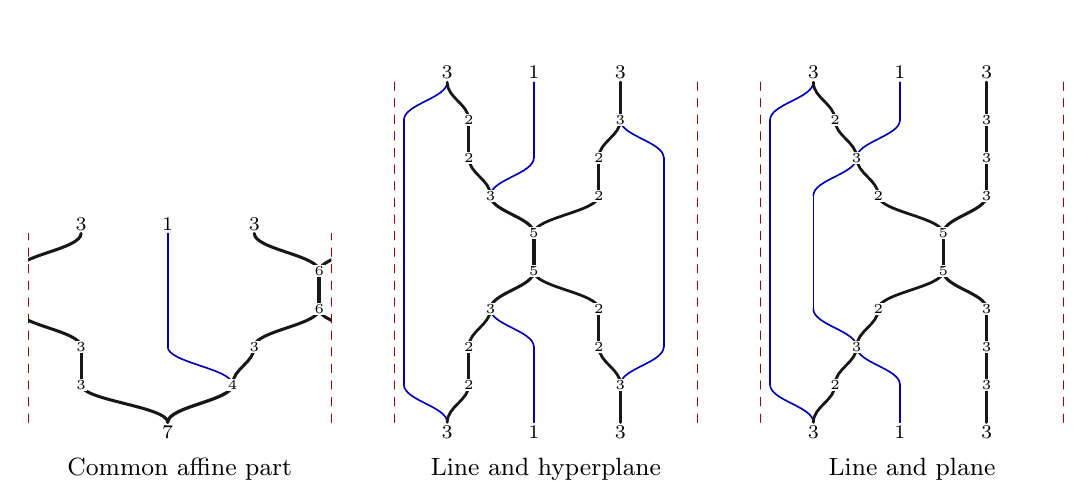
\begin{tikzpicture}[x=.55cm,y=.48cm,line cap=round,line join=round,baseline=(current bounding box.center)]
\begin{scope}[xshift=0cm]
\draw[red!68!black,dashed,thin] (.28,0)--(.28,5) (7.28,0)--(7.28,5);
\begin{scope}\clip (.28,-.18) rectangle (7.28,5.18);
\draw[black!91,line width=1.1042562584220408pt] (3.5,0) .. controls (3.5,0.42) and (1.5,0.58) .. (1.5,1);
\draw[black!91,line width=1.19pt] (3.5,0) .. controls (3.5,0.42) and (5.0,0.58) .. (5.0,1);
\draw[black!91,line width=1.1042562584220408pt] (1.5,1) .. controls (1.5,1.42) and (1.5,1.58) .. (1.5,2);
\draw[blue!74!black,line width=0.6pt] (5.0,1) .. controls (5.0,1.42) and (3.5,1.58) .. (3.5,2);
\draw[black!91,line width=1.1042562584220408pt] (5.0,1) .. controls (5.0,1.42) and (5.5,1.58) .. (5.5,2);
\draw[black!91,line width=1.1042562584220408pt] (1.5,2) .. controls (1.5,2.42) and (0.0,2.58) .. (0.0,3);
\draw[blue!74!black,line width=0.6pt] (3.5,2) .. controls (3.5,2.42) and (3.5,2.58) .. (3.5,3);
\draw[black!91,line width=1.1042562584220408pt] (5.5,2) .. controls (5.5,2.42) and (7.0,2.58) .. (7.0,3);
\draw[black!91,line width=1.1042562584220408pt] (8.5,2) .. controls (8.5,2.42) and (7.0,2.58) .. (7.0,3);
\draw[blue!74!black,line width=0.6pt] (3.5,3) .. controls (3.5,3.42) and (3.5,3.58) .. (3.5,4);
\draw[black!91,line width=1.333836717690617pt] (7.0,3) .. controls (7.0,3.42) and (7.0,3.58) .. (7.0,4);
\draw[black!91,line width=1.1042562584220408pt] (0.0,4) .. controls (0.0,4.42) and (1.5,4.58) .. (1.5,5);
\draw[blue!74!black,line width=0.6pt] (3.5,4) .. controls (3.5,4.42) and (3.5,4.58) .. (3.5,5);
\draw[black!91,line width=1.1042562584220408pt] (7.0,4) .. controls (7.0,4.42) and (5.5,4.58) .. (5.5,5);
\draw[black!91,line width=1.1042562584220408pt] (7.0,4) .. controls (7.0,4.42) and (8.5,4.58) .. (8.5,5);
\end{scope}
\node[fill=white,inner sep=.55pt,font=\tiny] at (1.5,1) {$3$};
\node[fill=white,inner sep=.55pt,font=\tiny] at (5.0,1) {$4$};
\node[fill=white,inner sep=.55pt,font=\tiny] at (1.5,2) {$3$};
\node[fill=white,inner sep=.55pt,font=\tiny] at (5.5,2) {$3$};
\node[fill=white,inner sep=.55pt,font=\tiny] at (7.0,3) {$6$};
\node[fill=white,inner sep=.55pt,font=\tiny] at (7.0,4) {$6$};
\node[below,inner sep=1pt,font=\scriptsize] at (3.5,0) {$7$};
\node[above,inner sep=1pt,font=\scriptsize] at (1.5,5) {$3$};
\node[above,inner sep=1pt,font=\scriptsize] at (3.5,5) {$1$};
\node[above,inner sep=1pt,font=\scriptsize] at (5.5,5) {$3$};
\node[below,align=center,font=\small] at (3.78,-.70) {Common affine part};\end{scope}
\begin{scope}[xshift=4.65cm]
\draw[red!68!black,dashed,thin] (.28,0)--(.28,9) (7.28,0)--(7.28,9);
\begin{scope}\clip (.28,-.18) rectangle (7.28,9.18);
\draw[blue!74!black,line width=0.6pt] (1.5,0) .. controls (1.5,0.42) and (0.5,0.58) .. (0.5,1);
\draw[black!91,line width=1.0025483399593904pt] (1.5,0) .. controls (1.5,0.42) and (2.0,0.58) .. (2.0,1);
\draw[blue!74!black,line width=0.6pt] (3.5,0) .. controls (3.5,0.42) and (3.5,0.58) .. (3.5,1);
\draw[black!91,line width=1.1042562584220408pt] (5.5,0) .. controls (5.5,0.42) and (5.5,0.58) .. (5.5,1);
\draw[blue!74!black,line width=0.6pt] (0.5,1) .. controls (0.5,1.42) and (0.5,1.58) .. (0.5,2);
\draw[black!91,line width=1.0025483399593904pt] (2.0,1) .. controls (2.0,1.42) and (2.0,1.58) .. (2.0,2);
\draw[blue!74!black,line width=0.6pt] (3.5,1) .. controls (3.5,1.42) and (3.5,1.58) .. (3.5,2);
\draw[black!91,line width=1.0025483399593904pt] (5.5,1) .. controls (5.5,1.42) and (5.0,1.58) .. (5.0,2);
\draw[blue!74!black,line width=0.6pt] (5.5,1) .. controls (5.5,1.42) and (6.5,1.58) .. (6.5,2);
\draw[blue!74!black,line width=0.6pt] (0.5,2) .. controls (0.5,2.42) and (0.5,2.58) .. (0.5,3);
\draw[black!91,line width=1.0025483399593904pt] (2.0,2) .. controls (2.0,2.42) and (2.5,2.58) .. (2.5,3);
\draw[blue!74!black,line width=0.6pt] (3.5,2) .. controls (3.5,2.42) and (2.5,2.58) .. (2.5,3);
\draw[black!91,line width=1.0025483399593904pt] (5.0,2) .. controls (5.0,2.42) and (5.0,2.58) .. (5.0,3);
\draw[blue!74!black,line width=0.6pt] (6.5,2) .. controls (6.5,2.42) and (6.5,2.58) .. (6.5,3);
\draw[blue!74!black,line width=0.6pt] (0.5,3) .. controls (0.5,3.42) and (0.5,3.58) .. (0.5,4);
\draw[black!91,line width=1.1042562584220408pt] (2.5,3) .. controls (2.5,3.42) and (3.5,3.58) .. (3.5,4);
\draw[black!91,line width=1.0025483399593904pt] (5.0,3) .. controls (5.0,3.42) and (3.5,3.58) .. (3.5,4);
\draw[blue!74!black,line width=0.6pt] (6.5,3) .. controls (6.5,3.42) and (6.5,3.58) .. (6.5,4);
\draw[blue!74!black,line width=0.6pt] (0.5,4) .. controls (0.5,4.42) and (0.5,4.58) .. (0.5,5);
\draw[black!91,line width=1.2655417527999329pt] (3.5,4) .. controls (3.5,4.42) and (3.5,4.58) .. (3.5,5);
\draw[blue!74!black,line width=0.6pt] (6.5,4) .. controls (6.5,4.42) and (6.5,4.58) .. (6.5,5);
\draw[blue!74!black,line width=0.6pt] (0.5,5) .. controls (0.5,5.42) and (0.5,5.58) .. (0.5,6);
\draw[black!91,line width=1.1042562584220408pt] (3.5,5) .. controls (3.5,5.42) and (2.5,5.58) .. (2.5,6);
\draw[black!91,line width=1.0025483399593904pt] (3.5,5) .. controls (3.5,5.42) and (5.0,5.58) .. (5.0,6);
\draw[blue!74!black,line width=0.6pt] (6.5,5) .. controls (6.5,5.42) and (6.5,5.58) .. (6.5,6);
\draw[blue!74!black,line width=0.6pt] (0.5,6) .. controls (0.5,6.42) and (0.5,6.58) .. (0.5,7);
\draw[black!91,line width=1.0025483399593904pt] (2.5,6) .. controls (2.5,6.42) and (2.0,6.58) .. (2.0,7);
\draw[blue!74!black,line width=0.6pt] (2.5,6) .. controls (2.5,6.42) and (3.5,6.58) .. (3.5,7);
\draw[black!91,line width=1.0025483399593904pt] (5.0,6) .. controls (5.0,6.42) and (5.0,6.58) .. (5.0,7);
\draw[blue!74!black,line width=0.6pt] (6.5,6) .. controls (6.5,6.42) and (6.5,6.58) .. (6.5,7);
\draw[blue!74!black,line width=0.6pt] (0.5,7) .. controls (0.5,7.42) and (0.5,7.58) .. (0.5,8);
\draw[black!91,line width=1.0025483399593904pt] (2.0,7) .. controls (2.0,7.42) and (2.0,7.58) .. (2.0,8);
\draw[blue!74!black,line width=0.6pt] (3.5,7) .. controls (3.5,7.42) and (3.5,7.58) .. (3.5,8);
\draw[black!91,line width=1.0025483399593904pt] (5.0,7) .. controls (5.0,7.42) and (5.5,7.58) .. (5.5,8);
\draw[blue!74!black,line width=0.6pt] (6.5,7) .. controls (6.5,7.42) and (5.5,7.58) .. (5.5,8);
\draw[blue!74!black,line width=0.6pt] (0.5,8) .. controls (0.5,8.42) and (1.5,8.58) .. (1.5,9);
\draw[black!91,line width=1.0025483399593904pt] (2.0,8) .. controls (2.0,8.42) and (1.5,8.58) .. (1.5,9);
\draw[blue!74!black,line width=0.6pt] (3.5,8) .. controls (3.5,8.42) and (3.5,8.58) .. (3.5,9);
\draw[black!91,line width=1.1042562584220408pt] (5.5,8) .. controls (5.5,8.42) and (5.5,8.58) .. (5.5,9);
\end{scope}
\node[fill=white,inner sep=.55pt,font=\tiny] at (2.0,1) {$2$};
\node[fill=white,inner sep=.55pt,font=\tiny] at (5.5,1) {$3$};
\node[fill=white,inner sep=.55pt,font=\tiny] at (2.0,2) {$2$};
\node[fill=white,inner sep=.55pt,font=\tiny] at (5.0,2) {$2$};
\node[fill=white,inner sep=.55pt,font=\tiny] at (2.5,3) {$3$};
\node[fill=white,inner sep=.55pt,font=\tiny] at (5.0,3) {$2$};
\node[fill=white,inner sep=.55pt,font=\tiny] at (3.5,4) {$5$};
\node[fill=white,inner sep=.55pt,font=\tiny] at (3.5,5) {$5$};
\node[fill=white,inner sep=.55pt,font=\tiny] at (2.5,6) {$3$};
\node[fill=white,inner sep=.55pt,font=\tiny] at (5.0,6) {$2$};
\node[fill=white,inner sep=.55pt,font=\tiny] at (2.0,7) {$2$};
\node[fill=white,inner sep=.55pt,font=\tiny] at (5.0,7) {$2$};
\node[fill=white,inner sep=.55pt,font=\tiny] at (2.0,8) {$2$};
\node[fill=white,inner sep=.55pt,font=\tiny] at (5.5,8) {$3$};
\node[below,inner sep=1pt,font=\scriptsize] at (1.5,0) {$3$};
\node[below,inner sep=1pt,font=\scriptsize] at (3.5,0) {$1$};
\node[below,inner sep=1pt,font=\scriptsize] at (5.5,0) {$3$};
\node[above,inner sep=1pt,font=\scriptsize] at (1.5,9) {$3$};
\node[above,inner sep=1pt,font=\scriptsize] at (3.5,9) {$1$};
\node[above,inner sep=1pt,font=\scriptsize] at (5.5,9) {$3$};
\node[below,align=center,font=\small] at (3.78,-.70) {Line and hyperplane};\end{scope}
\begin{scope}[xshift=9.3cm]
\draw[red!68!black,dashed,thin] (.28,0)--(.28,9) (7.28,0)--(7.28,9);
\begin{scope}\clip (.28,-.18) rectangle (7.28,9.18);
\draw[blue!74!black,line width=0.6pt] (1.5,0) .. controls (1.5,0.42) and (0.5,0.58) .. (0.5,1);
\draw[black!91,line width=1.0025483399593904pt] (1.5,0) .. controls (1.5,0.42) and (2.0,0.58) .. (2.0,1);
\draw[blue!74!black,line width=0.6pt] (3.5,0) .. controls (3.5,0.42) and (3.5,0.58) .. (3.5,1);
\draw[black!91,line width=1.1042562584220408pt] (5.5,0) .. controls (5.5,0.42) and (5.5,0.58) .. (5.5,1);
\draw[blue!74!black,line width=0.6pt] (0.5,1) .. controls (0.5,1.42) and (0.5,1.58) .. (0.5,2);
\draw[black!91,line width=1.0025483399593904pt] (2.0,1) .. controls (2.0,1.42) and (2.5,1.58) .. (2.5,2);
\draw[blue!74!black,line width=0.6pt] (3.5,1) .. controls (3.5,1.42) and (2.5,1.58) .. (2.5,2);
\draw[black!91,line width=1.1042562584220408pt] (5.5,1) .. controls (5.5,1.42) and (5.5,1.58) .. (5.5,2);
\draw[blue!74!black,line width=0.6pt] (0.5,2) .. controls (0.5,2.42) and (0.5,2.58) .. (0.5,3);
\draw[blue!74!black,line width=0.6pt] (2.5,2) .. controls (2.5,2.42) and (1.5,2.58) .. (1.5,3);
\draw[black!91,line width=1.0025483399593904pt] (2.5,2) .. controls (2.5,2.42) and (3.0,2.58) .. (3.0,3);
\draw[black!91,line width=1.1042562584220408pt] (5.5,2) .. controls (5.5,2.42) and (5.5,2.58) .. (5.5,3);
\draw[blue!74!black,line width=0.6pt] (0.5,3) .. controls (0.5,3.42) and (0.5,3.58) .. (0.5,4);
\draw[blue!74!black,line width=0.6pt] (1.5,3) .. controls (1.5,3.42) and (1.5,3.58) .. (1.5,4);
\draw[black!91,line width=1.0025483399593904pt] (3.0,3) .. controls (3.0,3.42) and (4.5,3.58) .. (4.5,4);
\draw[black!91,line width=1.1042562584220408pt] (5.5,3) .. controls (5.5,3.42) and (4.5,3.58) .. (4.5,4);
\draw[blue!74!black,line width=0.6pt] (0.5,4) .. controls (0.5,4.42) and (0.5,4.58) .. (0.5,5);
\draw[blue!74!black,line width=0.6pt] (1.5,4) .. controls (1.5,4.42) and (1.5,4.58) .. (1.5,5);
\draw[black!91,line width=1.2655417527999329pt] (4.5,4) .. controls (4.5,4.42) and (4.5,4.58) .. (4.5,5);
\draw[blue!74!black,line width=0.6pt] (0.5,5) .. controls (0.5,5.42) and (0.5,5.58) .. (0.5,6);
\draw[blue!74!black,line width=0.6pt] (1.5,5) .. controls (1.5,5.42) and (1.5,5.58) .. (1.5,6);
\draw[black!91,line width=1.0025483399593904pt] (4.5,5) .. controls (4.5,5.42) and (3.0,5.58) .. (3.0,6);
\draw[black!91,line width=1.1042562584220408pt] (4.5,5) .. controls (4.5,5.42) and (5.5,5.58) .. (5.5,6);
\draw[blue!74!black,line width=0.6pt] (0.5,6) .. controls (0.5,6.42) and (0.5,6.58) .. (0.5,7);
\draw[blue!74!black,line width=0.6pt] (1.5,6) .. controls (1.5,6.42) and (2.5,6.58) .. (2.5,7);
\draw[black!91,line width=1.0025483399593904pt] (3.0,6) .. controls (3.0,6.42) and (2.5,6.58) .. (2.5,7);
\draw[black!91,line width=1.1042562584220408pt] (5.5,6) .. controls (5.5,6.42) and (5.5,6.58) .. (5.5,7);
\draw[blue!74!black,line width=0.6pt] (0.5,7) .. controls (0.5,7.42) and (0.5,7.58) .. (0.5,8);
\draw[black!91,line width=1.0025483399593904pt] (2.5,7) .. controls (2.5,7.42) and (2.0,7.58) .. (2.0,8);
\draw[blue!74!black,line width=0.6pt] (2.5,7) .. controls (2.5,7.42) and (3.5,7.58) .. (3.5,8);
\draw[black!91,line width=1.1042562584220408pt] (5.5,7) .. controls (5.5,7.42) and (5.5,7.58) .. (5.5,8);
\draw[blue!74!black,line width=0.6pt] (0.5,8) .. controls (0.5,8.42) and (1.5,8.58) .. (1.5,9);
\draw[black!91,line width=1.0025483399593904pt] (2.0,8) .. controls (2.0,8.42) and (1.5,8.58) .. (1.5,9);
\draw[blue!74!black,line width=0.6pt] (3.5,8) .. controls (3.5,8.42) and (3.5,8.58) .. (3.5,9);
\draw[black!91,line width=1.1042562584220408pt] (5.5,8) .. controls (5.5,8.42) and (5.5,8.58) .. (5.5,9);
\end{scope}
\node[fill=white,inner sep=.55pt,font=\tiny] at (2.0,1) {$2$};
\node[fill=white,inner sep=.55pt,font=\tiny] at (5.5,1) {$3$};
\node[fill=white,inner sep=.55pt,font=\tiny] at (2.5,2) {$3$};
\node[fill=white,inner sep=.55pt,font=\tiny] at (5.5,2) {$3$};
\node[fill=white,inner sep=.55pt,font=\tiny] at (3.0,3) {$2$};
\node[fill=white,inner sep=.55pt,font=\tiny] at (5.5,3) {$3$};
\node[fill=white,inner sep=.55pt,font=\tiny] at (4.5,4) {$5$};
\node[fill=white,inner sep=.55pt,font=\tiny] at (4.5,5) {$5$};
\node[fill=white,inner sep=.55pt,font=\tiny] at (3.0,6) {$2$};
\node[fill=white,inner sep=.55pt,font=\tiny] at (5.5,6) {$3$};
\node[fill=white,inner sep=.55pt,font=\tiny] at (2.5,7) {$3$};
\node[fill=white,inner sep=.55pt,font=\tiny] at (5.5,7) {$3$};
\node[fill=white,inner sep=.55pt,font=\tiny] at (2.0,8) {$2$};
\node[fill=white,inner sep=.55pt,font=\tiny] at (5.5,8) {$3$};
\node[below,inner sep=1pt,font=\scriptsize] at (1.5,0) {$3$};
\node[below,inner sep=1pt,font=\scriptsize] at (3.5,0) {$1$};
\node[below,inner sep=1pt,font=\scriptsize] at (5.5,0) {$3$};
\node[above,inner sep=1pt,font=\scriptsize] at (1.5,9) {$3$};
\node[above,inner sep=1pt,font=\scriptsize] at (3.5,9) {$1$};
\node[above,inner sep=1pt,font=\scriptsize] at (5.5,9) {$3$};
\node[below,align=center,font=\small] at (3.78,-.70) {Line and plane};\end{scope}
\end{tikzpicture}

\end{center}
{\small Cut-open webs at $m=3$, read upwards. Stack the common part below either tail and identify each pair of red dashed sides. Blue strands have label one. The label-six strand in the common part straddles the cut. The vertices are the normalized splits and merges of A 2D.4.}\par

\noindent The product of the $2m-2$ individual simple KL elements
differs from the normalized completion for $m\ge3$.
At the identity coordinate, multiplication by $T_1T_2$ acts
by $[m]^2$, whereas the individual factors act by $\eta^{2m-2}$
(B, (3.4)). Since $\eps(\BS_m)\ne0$, evaluation at $v=1$ distinguishes
the two products by $m^2\ne4^{m-1}$ for $m\ge3$. Averaging further by
$C_V/\pi_V$ preserves this coordinate. At $m=2$ each parabolic
factor is already one simple KL element, so the raw products agree.

\clearpage
\subsection{Both finite tails are canonical}
\label{sec:finite-tails}

The finite tails can be compared in finite type~A before applying the
common affine prefix. In the finite spherical module $C_V\mathcal H(S_N)$ put
\[
 \mathsf a_m=\frac{C_VC_KC_V}{\pi_L^2},\qquad
 \mathsf b_m=\frac{C_VC_{K'}C_E}
 {\pi_{V\cap K'}\pi_{K'\cap E}}.
\]
The right $V$-eigenrelations of $F=C_IC_J/\pi_V$ define the module map
\[
 \Phi:C_V\mathcal H(S_N)\longrightarrow C_I\mathcal H(W),
 \qquad \Phi(C_Vh)=Fh.
\]
Thus $\Phi(\mathsf a_m)=\mathcal R_m$ and
$\Phi(\mathsf b_m)=\mathcal{BS}_m$, with all normalization factors included.
Both finite tails are single ordinary canonical elements:
\[
 \mathsf a_m=C_{w_A},\qquad
 w_A=w_0w_{\{s_m,s_{m+1}\}},
 \qquad
 \mathsf b_m=C_{w_B},\qquad
 w_B=[m,m+1,N,N-1,\ldots,m+2,m-1,\ldots,1].
\]
Their minimal left $V$-representatives have lengths $m^2+2m-3$
and $m^2-1$, respectively.

\noindent\textit{Proof.}
In the three-letter notation of the parabolic paper, let
$c_0=c_{\mathsf A^m\mathsf B\mathsf C^m}$, with window
$[1-m,\ldots,0,m+1,N+1,\ldots,N+m]$ and length $m^2$.
For $x\in{}^VW_I$, the map
$C_VH_x\mapsto M_{c_0x}$ identifies the finite standard basis with
the type-$m$ standard span. The window formula gives
$\ell(c_0x)=m^2+\ell(x)$, and the equal-letter and unequal-letter
multiplication rules show that it commutes with finite right Hecke
actions (B, Lemmas 3.8--3.9).
The type-$m$ part of $F$ is just $M_{c_0}$ with coefficient one
(B, Lemma 3.19).
Consequently the standard coefficients of the two finite tails are
exactly the type-$m$ coefficients of the two affine products.

At the boundary $m-r=0$, our six-family estimates give coefficient
one at the unique top and strictly positive valuation at every
proper orbit maximum; refinement adds the nonnegative length
deficit (A, Lemmas 4C.2 and 4D.1).
The lowest-exponent table in the parabolic paper at type $m$ has a unique $AB$ orbit
maximum of valuation zero; the $AA$ maxima have valuation one,
and every nonmaximum has an additional positive length deficit
(B, Proposition 3.21). The top coefficient is one in each case.
The two top words are $\mathsf C^{m-1}\mathsf A\mathsf B\mathsf C
\mathsf A^{m-1}$ and $\mathsf A\mathsf B\mathsf C^m\mathsf A^{m-1}$,
which give the displayed finite permutations. Integrality and bar
invariance of the normalized products now identify both tails by
canonical triangularity.\hfill$\square$

Let $L_m=C_{s_2}\cdots C_{s_m}C_{s_1}\cdots C_{s_{m-1}}$.
The corresponding reflection word takes $w_B$ to $w_A$, increasing
length at every step: first it moves $m+1$ past the larger entries,
then it moves $m$ past them. Finite KL multiplication therefore gives
\begin{align*}
 \mathsf b_mL_m
 &=\mathsf a_m+\sum_{z<w_A}d_z(v)C_z,
 &d_z(v)&\in\mathbb N[v,v^{-1}],\\
 \mathcal{BS}_mL_m
 &=\mathcal R_m+\sum_{z<w_A}d_z(v)\Phi(C_z).
\end{align*}
Only finite canonical indices with left $V$-descents occur in the sum.
The top multiplicity is one. This expresses our web as the image of
the top finite canonical summand after the two simple-reflection
chains. Using the normalized completion instead gives the exact
finite identity $\mathsf b_mT_1T_2=\mathsf a_m$.

For $m=3$, the correction has the following form. On the appropriate
spherical domain, the $S_3$ identity
$C_{\{s,t\}}=C_sC_tC_s-C_s$ gives
\[
 \mathcal R_3=\mathcal{BS}_3(C_2C_3-1)(C_1C_2-1),
 \qquad C_i=C_{s_i}.
\]
For $m=2,3,4,5$ the uncorrected finite product
$\mathsf b_mL_m-\mathsf a_m$ has respectively $0,3,10,20$
distinct canonical terms. These are exact finite checks; the
canonical-tail and summand statements above hold for all $m$.


\clearpage
\subsection{What the corrected seed contains}

Write $b_j=u_{j;m}^{-1}$ and let $[\,\C_b\,]$ denote a coefficient
in the spherical canonical basis. For every $1\le j\le m$,
\[
 \boxed{\ [\,\C_{b_j}\,](\C_{X_0}T_1T_2)=\delta_{jm}.\ }          \tag{**}
\]
At the other end of $(*)$, B, Proposition 3.21, also gives
$\BS_m=\sum_{j=1}^m\C_{z(j,1,0)}$. In fact its standards are in
$\mathbb Z[v]$, with constant term $1$ precisely at the $m$ indicated
orbit maxima and zero elsewhere. Subtracting those canonical elements
leaves a bar-invariant vector in $v\mathbb Z[v]\{M_c\}$, hence zero.
Thus $\R=\sum_{j=1}^m\C_{z(j,1,0)}T_1T_2$. In particular $(**)$
and A, Lemma 4I.1, place each off-diagonal family-F term, once, in
\[
 (\BS_m-\C_{X_0})T_1T_2
 =\Big(\BS_{m-1}-\eta\sum_{s=2}^{m-1}\CBS_s\Big)T_1T_2.
\]
Here $\BS_{m-1}$ is taken in the same period $2m+1$.

\smallskip
\noindent\textit{Proof of $(**)$.} For consecutive generators starting at
$s_a$ let $Z_0=Z$, $Z_i=Z C_{[a,a+i-1]}/\Pi_i$; assume $ZH_s=v^{-1}Z$
for $s\in[a+1,a+i-1]$. The left coset representatives are
$g_k=s_a\cdots s_{a+k-1}$, $0\le k\le i$, so that
\[
 Z_i=\sum_{k=0}^i v^{i-k}ZH_{g_k},
 \quad Z_1=ZC_{s_a},\quad
 Z_i=Z_{i-1}C_{s_{a+i-1}}-Z_{i-2}\quad(i\ge2).
\]
The last generator commutes with $g_k$ for $k\le i-2$, giving the
last recurrence. In B, Proposition 2.8, this subtracts the preceding
cover at each step. The remaining terms $\C_e,\C_{\gamma_k}$ are
eigenvectors for every later generator, since the word for $\gamma_k$
is $BC^kB^{N-2k-1}A^k$. Using $[i+1]=\eta[i]-[i-1]$ gives
\[
 \C_{X_0}T_1=\C_{x_{m-1}}+[m-1]\C_e+
             \sum_{k=1}^{m-2}[m-1-k]\C_{\gamma_k}.
\]
The terms after $\C_{x_{m-1}}$ retain the right descent $s_{m+1}$
upon multiplication by $T_2$, as $s_{m+1}$ commutes with $Q_2$.
Applying the same recurrence to B, Proposition 2.11, yields
\[
 \C_{x_{m-1}}T_2=\C_{\beta_m}+\sum_{t=0}^{m-2}[t+1]\mathcal E_t .
\]
Indeed each canonical term of $\mathcal E_t$ is sorted on its first
$m+1$ positions by B, Lemma 4.12(ii) and (4.17)--(4.18). Every
subsequent generator acts by $\eta$, and each such term has right
descent $s_m$. The canonical basis of the right $s$-spherical
subspace consists of the canonical elements with right descent $s$.
The word of $b_j$ is
$C^{j-1}B^{m-j}A\,|\,B\,|\,CB^{m-j}A^{j-1}$.
The adjacent ascents $AB,BC$ give both missing right descents
$s_m,s_{m+1}$ (B, Lemma 4.9). Therefore none of the remainders
contains any $\C_{b_j}$.\hfill$\square$

\smallskip
By B, Proposition 2.6, the identity coordinate of $\C_{X_0}T_1T_2$
has valuation $3-2m$. For $\C_{\beta_m}$ the valuation is one, so the
full vectors differ. Formula $(**)$ isolates the diagonal within family F.
Section~\ref{sec:partialrows} computes the degree-one identity coordinate
of each family-F constituent by completing successive partial sums.

\newpage
\section{Two ways of organizing the coefficient calculation}

Both arguments use the same refinement identity. If \(z\) is the longest index in a right-parabolic orbit, the coefficient of \(M_c\) in a vector invariant under that parabolic is \(v^{\ell(z)-\ell(c)}\) times its coefficient at \(z\). One proves this along a single edge by the quadratic Hecke relation. We use the identity to refine output flags (A, Lemma 4D.1). Bowman, de la Fuente, Libedinsky and Plaza use it to compute once per orbit (B, Lemmas 3.11, 3.17 and Proposition 3.21).

\paragraph{Two multiplicity-one expansions.}
The uncorrected product has a multiplicity-one expansion. Write \(z(t,a,b)\) for the longest element of their orbit of type \(t\) with indicators \(a,b\) for the first two letters. Then
\[
 \mathcal{BS}_m=\sum_{t=1}^m\mathbf C_{z(t,1,0)},\qquad
 \mathcal{BS}_{m-1}-\eta\sum_{s=2}^{m-1}\mathcal{CBS}_s
    =\sum_{t=1}^{m-1}\mathbf C_{z(t,1,0)},\qquad \eta=v+v^{-1}.
\]
Indeed, B Proposition 3.21 gives least exponents \(1,1,0,1\) at feasible maxima with prefixes \(BB,BA,AB,AA\), respectively, for \(\mathcal{BS}_m\). The \(AB\) maxima occur exactly for \(1\le t\le m\), and their constant terms are one. All other standard coordinates have positive valuation by refinement. Subtract the canonical vectors displayed in the first sum. The difference is bar invariant and every standard coordinate lies in \(v\mathbb Z[v]\), so it vanishes (B Lemma 3.1). B Proposition 3.5, with \(X_0=z(m,1,0)\), gives the second equality. In its proof the \(AB\) constants below the top cancel against \(\mathcal{BS}_{m-1}\); in column \(AA\) the \(-v^{-1}\) from that subtraction is canceled by \(+\eta\mathcal{CBS}_t\) at each type \(2\le t<m\). This isolates a single seed.

We prove multiplicity one for the completed web. In A, Lemma 3C.3, we fix flags \(I_0\subset K_0\) of dimensions \(r,N-r\) and \(F\subset F'\) of dimensions \(m,m+1\). For a line \(L\subset F\) and a hyperplane \(H\supset F'\), put \(e=\mathbf1_{L\not\subset I_0}\), \(d=\mathbf1_{H\not\supset K_0}\). The remaining choices of \(I'\subset K'\) of dimensions \(m,m+1\), between \(I_0+L\) and \(K_0\cap H\), number
\(
 \gb{N-2r-e-d}{m-r-e}_q(m+1-r-d)_q
\)
over a field of size \(q\). Sum against the corresponding line and hyperplane counts (A (3C.2)), substitute \(q=v^{-2}\) and multiply by \(v^{D-d_A}\), \(D=2m^2+2m-3\) (A Proposition 3C.4). If \(F_A(q)\) is the resulting counting polynomial before normalization, the exponents of a nonzero canonical multiplicity lie between \(-E\) and \(E\), \(E=2\deg F_A-(D-d_A)\). We apply positivity after clearing the overlap denominator. With \(l=m-r\), the bounds for the six allowed families A--F are respectively \(2l-3,l-2,l-1,l-2,l-1,0\) (Lemmas 4B.1 and 4C.2). At an F-standard \(A_{j;m}\), a full-spherical, strong one-incidence or weak one-incidence contribution of rank \(j+h\) starts in degree at least \(2h+6,2h+2,2h+4\), respectively. Larger F-terms contribute only positive powers there. Thus the constant one belongs to \(A_{j;m}\) itself (Lemma 4I.1). At a full-spherical standard, in contrast, one-incidence terms with their multiplicities start in degree at least three (Lemma 4H.1), which suffices for the row sum.

\newpage\subsection*{The same Gaussian and different subtractions}
The common Gaussian has a direct flag-counting explanation.
At the zero orbit, our gallery chooses
$L\subset I'\subset K'\subset H$ of dimensions $1,m,m+1,2m$,
with $L\subset F$ and $F'\subset H$, where
$\dim F=m$ and $\dim F'=m+1$.
There are $(m)_q$ choices each for $L$ and $H$.
In the $(2m-1)$-space $H/L$, the remaining flag
$I'/L\subset K'/L$ contributes
$\gb{2m-1}{m-1}_q(m)_q$.
The full count is therefore $(m)_q^3\gb{2m-1}{m-1}_q$.

Let \(t=v^2\), \(G=\gb{2m-1}{m-1}_t\), and use \((k)_t=1+\cdots+t^{k-1}\), \([k]=v^{1-k}(k)_t\). At the identity the normalized raw values are
\[
 \epsilon(\mathcal R_m)=v^{3-2m}(m)_t^3G,\qquad
 \epsilon(\mathcal{BS}_m)=v(m)_tG .
\]
These instances of the same rectangle follow from the operator identity and the finite eigenvalue, with ratio \([m]^2\) (A Prop.\ 3C.4, B proof of Prop.\ 2.6 in \S3.5). The auxiliary operators satisfy related identities after merging all outputs. Define \(U_j=C_I C_{J_j}C_I/\pi_{I\cap J_j}^2\) and let \(V_s=C_I C_{P_s}C_I/\pi_{I\cap P_s}^2\) be our spherical web (Definition 4E.1). With \(p_E(F)=FC_I/\pi_E\),
\[
 p_E(\mathcal{BS}_j)=[j]^2U_j,\qquad p_E(\mathcal{CBS}_s)=[s][s-1]V_s .
\]
Indeed \(C_Q C_I=\pi_Q C_I\) for \(Q\subset I\). The two factorial ratios remaining are \(\pi_{I\cap J_j}\pi_{K_j}/(\pi_{J_j\cap K_j}\pi_{K_j\cap E})=[j]^2\) and \(\pi_{I\cap P_s}/\pi_{P_s\cap E}=[s][s-1]\). Thus the parabolic seed correction includes scalar multiples of our cumulative spherical webs after the total merge. If instead one merges first to $Q=I\setminus\{s_1\}$ and appends the move to $I\setminus\{s_f\}$ for $f=m,m+1$, the result for $\CBS_s$ is $[s-1]$ times our one-line gallery $\mathcal E_{s,f}$. This follows from $\pi_{P_s\cap Q}/\pi_{P_s\cap E}=[s-1]$ and A Definition 4F.1.

We take the differences \(C_{Z_s}=V_s-V_{s-1}\), whose standard coefficients are differences of consecutive Gaussians (Lemma 4E.4). We subtract \(g_{m-s}C_{Z_s}\), where \(g_l=\sum_{a=0}^{l-2}\binom{a+3}{3}(v^{2l-3-2a}+v^{-(2l-3-2a)})\). To determine these multiplicities, we invert a convolution of Gaussian polynomials and truncate modulo \(q^m\); the common series \(1/((1-q)^3(q;q)_\infty)\) cancels, leaving \(\binom{m+1}{2}q^{m-1}\) (Lemmas 4J.1--4K.1). The surviving linear coefficient at the origin is the sum over family F (Theorem 4L.1).

In the parabolic paper the authors apply \(\epsilon\) to their corrected seed to obtain \(h_{X_0}=vG+O(v^{2m+1})\). The first \(m\) coefficients are ordinary partition numbers, since partitions of size below \(m\) fit the Gaussian rectangle. The first reflection chain satisfies \(h_{x_1}=\eta h_{X_0}-1\) and
\[
 h_{x_{k+1}}=\eta h_{x_k}-h_{x_{k-1}}-v^k\gb{N-1}{k}_t
 \quad(1\le k\le m-2).
\]
The last term is \(h_{\gamma_k}\) (Lemma 3.25). Bruhat covers supply the predecessor; positivity excludes the lower \(\gamma_j\), paired deletion reduces the surviving multiplicity to one, and a nonidentity seed bound excludes the \(\kappa_j\) (Proposition 2.8, Lemmas 3.24, 4.20, 5.1). If \(d_{a,b}\) counts partitions of \(a+b\) with at least \(a\) parts, the coefficient of \(v^{a+1+2b}\) in \(h_{x_a}\) is \(\sum_{i=0}^a d_{i,b}\) for \(0\le b\le m-1-a\) (Lemmas 2.9, 5.2). In particular \(h_{x_{m-1}}\) starts with \(mv^m\).

On the second chain the predecessor and remainder have identity-coordinate valuation at least \(t'+3\) in the step to \(y_{t'}\) (Proposition 2.11 and Lemma 2.12). Of its noncover candidates the ordered terms vanish after rank reduction, the pure terms have sufficiently high valuation by finite ascent bounds, and mixed terms vanish after a rank-two star operation and a descent test (Lemmas 6.1, 6.2, 6.5). This transports \(m\) down one degree at each step. They illustrate the remainders by explicit computation at \(m=5\) and prove the degree bound in every rank. Their partition recurrence follows the coefficient along a chain. Our
Gaussian convolution computes the row sum from the six-family base change.
The completion identity relates the products underlying these two calculations.

\paragraph{Relation to Scott--Xi.}
Scott--Xi, arXiv:0909.3394v4, Theorem 3.3, obtained \(n+2\) for \(\mu(xw_0,vxw_0)\) with a regularly translated lower endpoint. For the word in their Lemma 3.4 the fixed-source coefficient is \(2\) in every rank \(n\ge4\). At \(n=4\) this gives the \(m=2\) example in both papers. Scott--Xi pose the fixed-source question in Section 4. Their suggested weight for \(n=4k\) has coefficient \(p-2\) at every internal node, so for \(n>4\) it differs from the common diagonal weight considered here. The low-rank coincidence, the fixed-source question and the use of degree bounds in a KL recursion all have this earlier precedent.

\newpage
\begingroup
\setlength{\parskip}{.32em}
\setlength{\abovedisplayskip}{7pt plus 2pt minus 3pt}
\setlength{\belowdisplayskip}{7pt plus 2pt minus 3pt}
\section{Every entry of the row}
\label{sec:partialrows}
Combining our six-family bounds with the parabolic orbit estimates in B and applying the normalized completion gives
\[
                 \boxed{\ \mu_{j;m}=j\quad(1\le j\le m).\ }
\]
The proof takes the first \(j\) canonical summands of \(\mathcal{BS}_m\)
and applies \(T_1T_2\), with the ambient rank and our output boundary fixed.

\paragraph{1. Nested canonical sums before completing the web.}
Hereafter $\operatorname{val}$ denotes the lowest exponent of $v$, with $\operatorname{val}0=+\infty$. Let \(T=T_1T_2\) be the normalized finite tail which gives \(\mathcal{BS}_m T=\mathcal R_m\).
We use their notation for the longest orbit representatives and put
\[
 X_i=\mathbf C_{z(i,1,0)},\qquad D_s=\mathbf C_{z(s,1,1)},\qquad
 \Phi_j=\sum_{i=1}^j X_i,\qquad Y_j=\Phi_j T,\qquad Y_0=0 .
\]
Here \(X_i\) is a vector. The lower-case \(x_i\) in the parabolic paper is a permutation on a reflection chain.
We show
\begin{equation}\label{eq:partial-seeds}
 \mathcal{BS}_j=\Phi_j+\sum_{s=2}^{\min(j,m-1)}a_{js}(v)D_s,\qquad
 D_s=\mathcal{CBS}_s,\qquad
 \operatorname{val}a_{js}\ge 2-N+2j\quad(a_{js}\ne0).
\end{equation}
Only \(s\le m-1\) is needed: at \(j=m\) every \(a_{js}=0\). For \(s\le m-1\) B Proposition 3.21 gives \(\mathcal{CBS}_s\) a unique coordinate with nonpositive valuation: at the \(AA\) maximum of type \(s\), its constant is one. All others are positive, including nonmaxima by refinement. This proves its canonicality. The \(\mathcal{BS}_j\) are right \(E\)-invariant, so only maxima of \(E\)-orbits can be canonical indices; this is the parabolic canonical basis, or follows by descending triangularity in the invariant subspace. Outside the support listed in B Proposition 3.21 no canonical term can occur: clearing the Poincar\'e denominator gives a positive product in the ordinary KL basis. Apply the same valuation argument as A Lemma 4B.1 at the maxima. Columns \(BB,BA\) have positive valuation. Column \(AB\) has valuation zero, so its canonical multiplicity is constant. Column \(AA\) gives the bound \(2-N+2j\) in \eqref{eq:partial-seeds}. At an \(AB\) maximum of type \(i\) the coordinate of \(D_s=\mathcal{CBS}_s\), when present, has valuation \(N-2i\) by the same table. Multiplied by \(a_{js}\) it starts no lower than \(2+2(j-i)\). Other \(AB\) canonical vectors with constant multiplicities contribute only positive powers there. Thus the constant one belongs to \(X_i\) for every feasible \(1\le i\le j\). This proves \eqref{eq:partial-seeds} and in particular \(Y_m=\mathcal R_m\).

\paragraph{2. Support and multiplicity bounds.}
Each \(Y_j\) is integral and bar invariant. The domain of \(T\) is the right \(E\)-invariant module; both normalized factors are integral sums over finite parabolic cosets there (B Lemma 3.3). If \(p=(\Pi_{m-1})^2\) is their common denominator, \(p(Y_j-Y_{j-1})=X_j C_{Q_1} C_{Q_2}\) has nonnegative ordinary canonical coefficients. Consequently the cleared coefficient of \emph{each} \(Y_j\) is bounded coefficientwise by that of \(p\mathcal R_m\). Thus every canonical index of \(Y_j\) belongs to one of our six families. The valuation of a nonzero multiplicity is at least the corresponding valuation for \(\mathcal R_m\), by subtracting \(\operatorname{val}p\) from the inequality for cleared coefficients. This proves that the degree margins in A Lemmas 4H.1 and 4I.1 apply to \(Y_j\) as well. In particular, for each family-F index its multiplicity in \(Y_j\) is a constant zero or one, nondecreasing in \(j\), since its multiplicity in \(\mathcal R_m\) is one. All standard and canonical indices of \(Y_j\) have type at most \(j\): \eqref{eq:partial-seeds} and B Proposition 3.21 bound the initial standard support, finite right generators preserve word type, and positivity after clearing excludes any additional canonical support.

For completeness we compute the constant at \(A_{j;m}\). A flag for \(\mathcal{BS}_jT\) chooses intermediate \(U\subset U'\) of dimensions \(j,j+1\), with \(I_0\subset U\subset U'\subset K_0\), in the finite quotient of A Definition 3C.1. To check the input conditions directly, B Lemma 3.19 restricts the first parabolic product to words whose $\mathsf A$ letters are in the first \(j\) positions, whose singleton is neutral and whose $\mathsf C$ letters are after position \(j+1\). On the rank orbit this says precisely \(I_0\subset U\subset U'\subset K_0\). The one-cut product similarly imposes just \(I_0\subset U\subset K_0\). Equivalently, divide the nested periodic lattices by the final lattice as in our proof of Proposition 3C.4 in A. For the output \(F\subset F'\) of dimensions \(m,m+1\), it also chooses a line \(L\subset U\cap F\) and a two-plane \(D\) with \(L\subset D\subset U'\cap F'\). Indeed the flags between the first affine parabolic and the output successively retain \((L,U')\), \((L,D)\), \((L,F')\); this works also when \(j=1\) with the repeated cut suppressed. For \(\mathcal{CBS}_s T\), the first affine parabolic retains just an \(s\)-space \(U\) with \(I_0\subset U\subset K_0\), and the final conditions become \(L\subset F\), \(L\subset D\subset U\cap F'\).

At \(A_{j;m}\) the rank is \(j\), so \(U=I_0\) in the first gallery. A Lemma 4C.2 gives \(\dim(I_0\cap F)=\dim(I_0\cap F')=1\) and \(\dim(K_0\cap F')=m-j+2\). Thus \(L\) is forced. The line \(U'/I_0\) must belong to the image of \(K_0\cap F'\) modulo \(I_0\); then \(U'\cap F'\) is the unique possible \(D\). The count is \((m-j+1)_q\) where \(q\) is the flag parameter. Its normalization shift is \(2(m-j)\): the gallery normalization constant is
\[
 d_j^{\rm BS}=4m-3+2(j-1)(N-j-1),
\]
as follows either by summing the parabolic length shifts or by the origin count below, and A Lemma 4C.2 gives \(d_{A_{j;m}}=2j(N-j)-2(m-j)-3\). Thus the normalized coordinate has constant one. For \(\mathcal{CBS}_sT\), \(s<j\) is impossible and \(s=j\) would require \(D\subset I_0\cap F'\), also impossible. The constant therefore belongs to \(Y_j\). By the margins of A Lemma 4I.1 it is the multiplicity of \(C_{A_{j;m}}\). Monotonicity and the type bound now show that the family-F indices occurring in \(Y_j\) are exactly \(A_{1;m},\ldots,A_{j;m}\), once each.

\paragraph{3. Coordinates at the full-spherical standards.}
At \(Z_r\) we have \(I_0\cap F'=0\), \(\dim(F\cap K_0)=m-r\), and \(\dim(F'\cap K_0)=m-r+1\), by A Definition 3C.1 and Lemma 4C.2. The choices of \(L,D\) in \(K_0\) number \((m-r)_q^2\), and \(D\) is disjoint from \(I_0\). For the BS gallery choose \(U'/I_0\) containing the image of \(D\), then a hyperplane \(U/I_0\) containing the image of \(L\). For the CBS gallery choose \(U/I_0\) containing the image of \(D\). The two flag counts are, respectively,
\[
 (m-r)_q^2(j-r)_q\gb{N-2r-2}{j-r-1}_q,\qquad
 (m-r)_q^2\gb{N-2r-2}{s-r-2}_q.
\]
The first vanishes for \(r\ge j\), the second for \(r>s-2\); these cases are omitted before evaluating Gaussians. The standard normalization is \(v^{d-d_{Z_r}}\) times the count at \(q=v^{-2}\), where \(d_{Z_r}=2r(N-r)\) in our normalization. To verify the absolute shifts, use the origin formulas in B, proof of Proposition 2.6, multiplied by \([m]^2\) for \(T\). Reversing the displayed counting polynomials at \(r=0\) gives \(d=d_j^{\rm BS}\) as above and \(d=d_s^{\rm CBS}=6m-2s+2(s-2)(N-s)\). The flag normalization depends on the endpoint standard only through \(d_{Z_r}\) (A Lemmas 2D.4, 2E.3). Subtracting \(2r(N-r)\) in either formula amounts to replacing \((m,j,s,N)\) by \((m-r,j-r,s-r,N-2r)\).

Set \(h=j-r>0\), \(t=v^2\). On its support the BS coordinate is therefore
\[
 v^{3-2h}(m-r)_t^2(h)_t\gb{2(m-r)-1}{h-1}_t .
\]
The corresponding CBS coordinate has valuation \(2m+4-2s\); by \eqref{eq:partial-seeds} its contribution to \(Y_j\) starts no lower than \(5+2(j-s)\). Consequently, through degree one inclusive, the \(Z_r\)-coordinate of \(Y_j\) agrees with the \(Z_r\)-coordinate of \(\mathcal R_j\) in \emph{ambient parameter \(j\)}. Indeed \((m-r)_t\equiv(h)_t\bmod t^h\); both Gaussian numerators in the rectangle product formula start contributing only in degree \(h\) or higher. Multiplication by \(v^{3-2h}\) puts the error in degree at least three. For \(r\ge j\) these coordinates vanish.

\paragraph{4. The same spherical corrections in the smaller parameter.}
For \(r\le s\le j\), the \(Z_r\)-coordinate of the canonical \(C_{Z_s}\) is
\[
 \gb{2(m-r)+1}{s-r}_t-\gb{2(m-r)+1}{s-r-1}_t
\]
(A Lemma 4E.4). It agrees modulo \(t^{j-r+1}\) with the same coordinate in ambient parameter \(j\): in both rectangle formulas the first numerator exponent is at least \(j-r+2\), unless the lower entry is negative, in which case the Gaussian is zero. In particular, for \(s\le j-2\) this agreement persists through degree one after multiplication by our correction \(g_{j-s}\), whose valuation is \(3-2(j-s)\).

For \(r\ge j\), the standard coordinates at \(Z_r\) vanish;
positivity after clearing the denominator excludes the corresponding
full-spherical canonical summands. At \(r=j-1\) the coordinate starts
in degree one, so its bar-symmetric spherical multiplicity is zero.
Now descend through \(r\le j-2\). At \(Z_r\) all one-incidence terms in \(Y_j\), including their multiplicities, have valuation at least three (step 2 and A Lemma 4H.1). Every family-F coefficient there is proper, hence has positive valuation, and its multiplicity is constant. Full-spherical indices of rank less than \(r\) have zero coordinate. Thus after subtracting the already known higher full-spherical terms, the nonpositive powers at \(Z_r\) determine its bar-symmetric multiplicity completely. By step 3 and the preceding Gaussian comparison these powers agree with our smaller-parameter computation (Lemmas 4J.2, 4K.1). It follows that the multiplicity at \(Z_r\) in \(Y_j\) is \(g_{j-r}\) for \(0\le r\le j-2\), and zero for \(r\ge j-1\). At \(r=0\), after all these subtractions the coefficient of \(v\) is also the one in our smaller calculation, namely \(\binom{j+1}{2}\). For \(j=1\), the raw coordinate begins with \(v\), and there is no spherical subtraction; this gives the same formula directly.

The only remaining contributors in degree one at \(Z_0\) are the family-F terms of step 2. We have proved \(\sum_{i=1}^j\mu_{i;m}=\binom{j+1}{2}\) while \emph{holding \(m\) fixed}. Taking consecutive differences gives the individual formula.

Equivalently, before reading the distinguished coefficient, \(X_iT=Y_i-Y_{i-1}\) contains \(C_{A_{i;m}}\) once and none of the other family-F vectors. Its full-spherical coefficient at \(Z_r\) is \(g_{i-r}-g_{i-1-r}\), with \(g_a=0\) for \(a\le1\). The residual one-incidence terms can persist as operators. Their origin coordinates, including multiplicities, start in degree at least three by the same cleared-positivity bound. We thus identify one canonical summand in the parabolic product for each entry of our row.
\label{partial:end}
\par\endgroup

\newpage
\section{The first-entry polynomial and rank reduction}
Put \(b_{j;m}=u_{j;m}^{-1}\) and \(h_x=[M_e]\mathbf C_x\). In the word convention of the parabolic paper,
the negative, zero and positive shifts in our sorted window give the letters
\(\mathsf C,\mathsf B,\mathsf A\), respectively. Thus the word of \(b_{j;m}\) is
\[
 \mathsf C^{j-1}\mathsf B^{m-j}\mathsf A\mathsf B\mathsf C
                  \mathsf B^{m-j}\mathsf A^{j-1}.
\]
The two reflection chains in that paper keep \(m\) letters of each wound type throughout.
The off-diagonal endpoints have \(j<m\) of each.

\subsection*{The first entry admits a finite Hecke calculation}
\textbf{Deduction.} For every \(m\ge2\),
\[
   P_{w_0,C_{1;m}}(q)=1+q+\cdots+q^{m-1},\qquad \mu_{1;m}=1 .
\]
Indeed, the window of \(s_0\) has \(0\) at position \(1\) and \(N+1\) at
position \(N\). Moving them to positions \(m,m+2\) gives
\[
 b=b_{1;m}=s_0(s_1\cdots s_{m-1})(s_{N-1}\cdots s_{m+2})\in W_J .
\]
Use the same \(V=I\cap J\) and \(L=V\setminus\{s_1,s_{N-1}\}\) as in our gallery.
Thus \(W_V=S_m\times S_m\). Write \([a]=(v^a-v^{-a})/(v-v^{-1})\).
In the spherical right module consider the bar-invariant vector
\(G=M_e C_{s_0}C_V/\pi_L\), where \(C_V=C_{w_V}\).
The right \(W_V\)-orbit of the left coset indexed by \(s_0\) has minimal
index \(s_0\) and maximal index \(b\). Its elements move the one
\(\mathsf A\) within the first block of \(m\) positions and the one
\(\mathsf C\) within the last block, keeping the middle \(\mathsf B\) fixed.
The stabilizer is \(W_L\). Expanding the parabolic symmetrizer into
minimal coset representatives gives
\[
 G=\sum_{x\in\mathcal O_V(s_0)}
 v^{\ell(b)-\ell(x)}M_x+v[m]^2M_e .
\]
Here \(M_e C_{s_0}=M_{s_0}+vM_e\), and \(\pi_V/\pi_L=[m]^2\).
For the orbit term, each shortest shuffle moves the two marked letters
away from their initial positions by length-increasing steps. Thus it
acts by \(M_{s_0}H_z=M_{s_0z}\), with exponent
\(\ell(w_V)-\ell(w_L)-\ell(z)=\ell(b)-\ell(s_0z)\).
This is also the orbit formula underlying B \S3.3.
Now \(v[m]^2-[m][m-1]=v^m[m]\). The vector
\[
 \mathbf C_b=G-[m][m-1]M_e
\]
is characterized by bar invariance, leading standard \(M_b\) with
coefficient one, and strictly positive powers of \(v\) at all other
standards. This proves the displayed KL formula since
\(h_b=v^m[m]\) and \(\ell(b)=2m-1\).

This finite calculation gives the entire first-column KL polynomial. For example, at $m=3$ it gives $1+q+q^2$. Section~\ref{sec:partialrows} determines the leading coefficient of every column.


\subsection*{The first seed in the uncorrected parabolic family}
The same entry can be read from the parabolic product in the ambient period
\(2m+1\). With \(T_1,T_2\) as in \((*)\) and our strong one-line
canonical \(\mathcal E_{1,m}\) refined to \(V\), one has
\[
 \mathcal{BS}_1T_1T_2=\mathbf C_{b_{1;m}}+[m-1]\mathcal E_{1,m}.
\]
Here \(\mathcal{BS}_1=D(J_1)\) has coefficient \(v^{2m-1}\) at \(e\)
and \(v^{c-3}\) at the rank-one words with \(\mathsf A\) in position
one and \(\mathsf C\) in position \(3\le c\le N\) (B Lemma 3.19).
For the three output orbit maxima \(H,U,F\), the \(\mathsf A\) is in
position \(m\) and the \(\mathsf C\) in positions \(1,m+1,m+2\),
respectively. The four standard coordinates are
\[
\begin{array}{c|cccc}
 &H&U&F&e\\ \hline
 \mathcal{BS}_1T_1T_2 &[m-1]&v^{m-1}[m-1]&v^{m-1}[m]&v^{2m-1}[m]^2\\
 \mathcal E_{1,m} &1&v^{m-1}&v^m&v^{2m}[m].
\end{array}
\]
For the first row, \(T_1\) sends the terms \(3\le c\le m+1\) to
their orbit sum with top coefficient
\(\sum_{c=3}^{m+1}v^{c-3+c-m-1}=[m-1]\), and multiplies the others
by \([m]\). For \(H\), the second averaging contributes the sum
\(\sum_{c=2}^m v^{c-2+c-m}=[m-1]\) divided by \([m-1]\);
for \(U,F\) it moves a single \(\mathsf A\) to the end of the first
block. The second row follows from A Lemmas 4F.2 and 4D.1.
These are all occupied orbits. Subtract the rows with the stated factor,
using \(v^{m-1}[m]-v^m[m-1]=1\).

\newpage
\subsection*{The rank-reduction identity}
Let \(\Theta_k\) have word \(\mathsf C^k\mathsf B^{N-2k}\mathsf A^k\).
It is the finite-orbit maximum of type \(k\) (B Lemma 3.11), hence represents
our full-spherical standard \(Z_k\) after output refinement. The coefficient
at its longest fine representative has shift zero (A Lemma 4D.1).
For \(0\le k<j\le m\) we obtain the all-degree identity
\[
   [\Delta_{Z_k}]C_{A_{j;m}}
   =[M_{\Theta_k}]\mathbf C_{b_{j;m}}
   =h^{(m-k)}_{b_{j-k;m-k}},
\]
where the superscript gives the smaller rank parameter.
For \(k>0\), both ordinary endpoints \(w_I\Theta_k,w_Ib_{j;m}\) take
the values \(2N,1-N\) at positions \(1,N\), respectively. Every
fundamental-window entry lies between those bounds. Deleting the common
first and last letters removes one \(\mathsf C\) and one \(\mathsf A\):
the relabelling in B Definition 4.17 gives
\(w'_I\Theta_{k-1},w'_I b_{j-1;m-1}\), with period \(N-2\).
To check Bruhat comparability use the rank functions
\(\#\{i\le a:w(i)\ge b\}\).
At each cut the deleted periodic strands contribute equally to the
two functions. On the remaining strands their inequalities are exactly
the smaller-period inequalities. Iterating reaches the comparable pair
\(w'_I,w'_I b_{j-k;m-k}\). B Proposition 4.18 now applies at each
deletion and preserves the normalized coefficient. For \(j\le k\) the
original coordinate vanishes since
\(\ell(\Theta_k)=2k(N-k)\ge 2j(N-j)>D_{j;m}\).

On the diagonal, the coefficient formula in the parabolic paper gives \([v][\Delta_{Z_k}] C_{A_{m;m}}=m-k\) for
\(0\le k<m\). The final case reduces to \(s_0\) in period three.
The independent KL recursion checked the full polynomial identity for every
\(k,j\) in ranks \(m=2,3,4\). For example, at \(m=4\) the rows of
linear coefficients, with columns \(j=1,2,3,4\), are
\((1,2,3,4),(0,1,2,3),(0,0,1,2),(0,0,0,1)\).
Together with our one-line degree bound at each \(Z_k\) (Lemma 4H.1),
these tests at full-spherical standards recover the row sums in
parameters \(m-k\). To distinguish entries within a fixed row,
Section~\ref{sec:partialrows} computes its successive partial sums.

\subsection*{The length gap in direct rank reduction for \(2\le j<m\)}
At the ordinary pair \(w_I,w_Ib_{j;m}\) the only common window
position is the central \(\mathsf B\) at \(m+1\). The other two
\(\mathsf B\)-blocks have \(b(i)=i+1\) and \(i-1\), respectively.
Deleting the common position and image leaves type \(j\) in period
\(N-1\). In B Lemma 3.9, \(\ell=2j(N-j)-\operatorname{inv}\) with
\(\mathsf C<\mathsf B<\mathsf A\). Deletion drops two inversions, one
with the preceding \(\mathsf A\), one with the following \(\mathsf C\).
The ordinary length gap therefore drops by \(2j-2>0\), preventing
Henderson cancellation at this strand. Across fixed \(j\) the full gap
difference is \(D_{j;m}-D_{j;j}=(4j-2)(m-j)\).

The seed correction also depends on the ambient parameter. B Proposition 3.21 gives
lowest exponent \(2-(N-2j)=1-2(m-j)<0\) for \(\mathcal{BS}_j\) at the
orbit maximum \(z(j,1,1)\). The terms \(\mathcal{BS}_{j-1}\) and
\(\mathcal{CBS}_s\) for \(s\le j-1\) vanish on this type-\(j\) orbit.
Replacing \(m\) by \(j\) in the correction while retaining period \(2m+1\)
therefore leaves a negative power at this orbit, so it does not give the
canonical seed.

\newpage\section{What follows for coefficients and cohomology}

Write \(k=\overline{\mathbb F}_p\), \(N=2m+1\), and \(G=\mathrm{SL}_N(k)\).
For degree one, both papers assume Lusztig's character formula in the
given rank and \(p\ge5(N-1)\) for finite group comparison. These assumptions
hold for every sufficiently large \(p\) at fixed \(m\).

\begingroup\small\renewcommand{\arraystretch}{1.17}
\begin{tabularx}{\linewidth}{@{}>{\raggedright\arraybackslash}p{.215\linewidth}Y@{}}
\toprule
Setting and source & Consequence \\ \midrule
A, Theorem 4L.1 and Corollary 6C.2 &
\(\sum_{j=1}^m\mu_{j;m}=m(m+1)/2\).
Each coefficient equals the rational \(H^1\)-dimension of
\(L(\lambda_{j;m}(p))\) and the finite \(H^1\)-dimension for its restriction
to \(\mathrm{SL}_N(\mathbb F_p)\) and its descendant \(M_{j;m}(p)\)
on \(\mathrm{PSL}_N(\mathbb F_p)\), over \(k\).
The row sum gives \(\max_j\mu_{j;m}\ge\lceil(m+1)/2\rceil\).\\
B, Theorems A and B &
\(\mu_{m;m}=m\), and
\(\dim_{\mathbb F_p}H^1(\mathrm{PSL}_N(\mathbb F_p),V_{m,p})=m\).
All \(V_{m,p}\) are faithful and absolutely irreducible.\\
The two KL theorems together &
\(\sum_{j<m}\mu_{j;m}=m(m-1)/2\) and \(\max_j\mu_{j;m}\ge m\).\\
Partial-row calculation, \S\ref{sec:partialrows} &
$\mu_{j;m}=j$ throughout, with maximum $m$ at $j=m$. For each sufficiently large $p$, our $m$ modules realize every first cohomology dimension $1,\ldots,m$ for this one finite group.\\
B, Theorem B, (2.17), Corollary 2.20 &
For \(0\le s<m\), the normalized polynomial for \(y_s\) starts with
\(mv^{s+1}\). For large \(p\),
\(\dim_k H^{s+1}(G,L(y_s\cdot_p0))=m\), and its rational
cohomology vanishes in all lower degrees. The identified diagonal is \(s=0\).\\
B, Theorem C, Lemma 2.18 &
Fix \(1\le n\le m\). For sufficiently large \(p\), then sufficiently
large \(a\), a faithful absolutely irreducible \(k\)-module for
\(\mathrm{PSL}_N(\mathbb F_{p^a})\) has \(\dim_kH^n\ge m\).
The proof uses injective restriction.\\
B, Theorem D, (2.18) &
For a primitive complex root of odd order \(\ell>N\),
\(\dim_{\mathbb C}H^{s+1}(U_\zeta,L_\zeta(y_s\cdot_\ell0))=m\),
with vanishing in lower degrees. This is Ext in finite-dimensional
integrable type-1 modules of Lusztig's divided-power quantum group.\\
A with B's (2.18) &
The same standard quantum KL formula transports our row sum to quantum
\(H^1\) for the \(m\) modules \(L_\zeta(u_{j;m}^{-1}\cdot_\ell0)\).\\
\bottomrule
\end{tabularx}\endgroup

\paragraph{The coefficient fields.}
On the diagonal the highest weights agree. The split group gives an
\(\mathbb F_p\)-form of the simple highest-weight module. Its root-lattice
weight makes the finite center act trivially. That center has
prime-to-\(p\) order, so inflation across it is an isomorphism in every
degree. Thus, as modules for the \emph{same} finite group,
\[
 M_{m;m}(p)\cong V_{m,p}\otimes_{\mathbb F_p}k.
\]
Extending the finite group bar complex shows that the scalar extension
preserves the cohomology dimension. The same descent applies to our
other restricted highest weights. See A Lemmas 6A.2, 6B.1 and 6C.1;
B Proposition 2.15 and the proof of Theorem A.

\paragraph{Finite-group comparison in higher degrees.}
For the weights in the parabolic paper, the standard large-characteristic comparison gives exact
finite-group cohomology dimensions.
Fix \(1\le n\le m\), set \(\lambda=y_{n-1}\cdot_p0\), and assume
the character-formula hypotheses in that paper together with
\(p\ge(4n+1)(N-1)\).
B Lemma~2.17 makes \(\lambda\) nonzero, \(p\)-restricted and a root-lattice
weight in the affine dot orbit of zero. It is therefore \(p^a\)-restricted
for every \(a\ge1\).
Parshall--Scott--Stewart, \emph{Shifted generic cohomology},
Theorem~5.12 and its proof on pp.~1780--1781, give
\[
 H^d(\mathrm{SL}_N(\mathbb F_{p^a}),L(\lambda))
 \cong H^d(G,L(\lambda))
 \qquad(1\le d\le n,\ a\ge1).
\]
Here one takes \(\nu=0\) in the Bendel--Nakano--Pillen
Theorem~7.5 comparison displayed in that proof.
Combining this with Theorem~B and (2.17) of the parabolic paper, and inflating across the
prime-to-\(p\) center, gives a faithful absolutely irreducible
\(k\mathrm{PSL}_N(\mathbb F_{p^a})\)-module \(V_a\) with
\[
 \dim_k H^n(\mathrm{PSL}_N(\mathbb F_{p^a}),V_a)=m,\qquad
 H^d(\mathrm{PSL}_N(\mathbb F_{p^a}),V_a)=0\quad(0\le d<n).
\]
Degree zero vanishes by nontrivial irreducibility.
In particular, equality and lower-degree vanishing hold for \(a=1\).
This follows from the rational cohomology calculation in the parabolic paper and the cited
comparison theorem.
The required lower bound on the characteristic depends on the rank and
the chosen degree.
\href{https://doi.org/10.1112/S0010437X13007331}{doi:10.1112/S0010437X13007331}.

\newpage
\section{Exact calculations in the spherical module}
\label{sec:checks}

The accompanying Python program implements two calculations over
$\mathbb Z[v,v^{-1}]$. In the first, represent a standard vector by the
levels $a_i=\lfloor(x(i)-1)/N\rfloor$ of the left-minimal window.
To apply $C_P/\pi_T$, where $T$ is the previous intersection, cut the
circle at a missing reflection and add one to the levels that pass the cut.
In each position block sort the lifted levels in increasing order. Let $L$
be the stabilizer of this minimum in $W_P$, $d(x)$ the within-block
inversion number and $D=\ell(w_P)-\ell(w_L)$. The new coefficient at $y$
in its orbit $O$ is
\[
 v^{D-d(y)}\frac{\pi_L}{\pi_T}\sum_{x\in O}v^{-d(x)}[M_x]F .
\]
Indeed $M_xC_P=v^{-d(x)}M_{\min O}C_P$ and splitting $W_P$ into
minimal left $W_L$-coset representatives evaluates the latter expression.
All Laurent divisions in the program check for zero remainder.

The second calculation uses only right simple reflections. For a right
descent $s$ of $x$, recursively calculate $\mathbf C_{xs}C_s$. At
each strict lower $z$ subtract the constant term of its standard
coordinate times $\mathbf C_z$. The resulting monic bar-invariant
vector satisfies the canonical triangularity condition. This recursion independently computes the seed in the parabolic paper, every endpoint, and the canonical transition matrix
used to decompose the products. The numerical inputs are the parabolic
sets, the chain words and the endpoint windows.

Let $L_m=C_{s_2}\cdots C_{s_m}C_{s_1}\cdots C_{s_{m-1}}$ and let
$D_m$ denote the two normalized parabolic averages. Each cell below
gives the degree-one identity coefficient followed by the number of
distinct canonical indices with nonzero graded multiplicity.
\begin{center}
\begin{tabular}{c|ccccc}
$m$ & $\mathcal R_m$ & $\mathcal{BS}_m L_m$ &
$\mathbf C_{X_0}L_m$ & $\mathbf C_{X_0}D_m$ & $\mathbf C_{\beta_m}$\\ \hline
2 & $4,5$ & $4,5$ & $3,3$ & $3,3$ & $2,1$\\
3 & $11,11$ & $18,23$ & $12,13$ & $7,6$ & $3,1$\\
4 & $25,17$ & $81,70$ & $50,38$ & $14,9$ & $4,1$
\end{tabular}
\end{center}
In each rank all five columns have identical standard support,
respectively $38,368,3098$ indices, and coefficient one at $M_{\beta_m}$.
Every coordinate of $\mathcal{BS}_mD_m$ agrees with $\mathcal R_m$.
Of the family-F summands, the first two columns contain the entire row
with multiplicity one, and the diagonal is the unique family-F term in the last three.
The independent KL recursion gives rows $(1,2),(1,2,3),(1,2,3,4)$.
For instance
\[
 [M_e]\mathbf C_{\beta_2}=2v+4v^3+5v^5+4v^7+v^9,\qquad
 [M_e]\mathbf C_{X_0}=v+v^3+2v^5+v^7\quad(m=2).
\]
Executing \texttt{python3 compare.py --full 2 3 4} in the directory
containing \texttt{compare.py} reproduces the tables and full identity
polynomials in \texttt{results.txt} without external packages. A second
script, \texttt{python3 partial.py 2 3 4 5}, checks the mixed
full-spherical coordinates and the discarded degrees directly. In rank
five its successive corrected degree-one coefficients are $1,3,6,10,15$;
the independent KL recursion gives $(1,2,3,4,5)$. For selected entries at larger values of $m$, a separate run gives $\mu_{2;6}=\mu_{2;7}=\mu_{2;8}=2$, $\mu_{3;6}=\mu_{3;7}=3$ and $\mu_{4;6}=4$. The last expansion has 120\,862 standard terms. The script \texttt{check\_off\_diagonal.py} and its output accompany the calculation.

\paragraph{Comparison after boundary projection.}
At $m=2$, $L_m=D_m$. For $m\ge3$, applying the projector $C_V/\pi_V$ to
$\mathcal{BS}_mL_m$ gives a vector linearly independent of
$\mathcal R_m$ over $\mathbb Q(v)$. It suffices to compare two
coordinates at $v=1$. Write $t=2^{m-1}/m$. The ratio at $M_e$ is
$t^2$ since each simple factor multiplies this coordinate by 2,
whereas each divided parabolic factor multiplies it by $m$.
The ratio at $M_{\beta_m}$ is $t$, as follows.

In type $m$ the first affine product has just the word $A^mBC^m$.
The next $K_m$-average fixes the initial $A$ and puts the $B$ in any
one of positions $2,\ldots,m+1$. The $E$-average then gives coefficient
one to every type-$m$ word with prefix $AB$ (the stabilizer of the
remaining letters has size $(m-1)!m!$, exactly the overlap denominator).
The last $m$ letters stay fixed during $L_m$. In the $V$-orbit of
$\beta_m$ they contain one $C$ and $m-1$ letters $A$, so only
the initial prefix $ABC^{m-1}$ of length $m+1$ can contribute:
the leftmost letter is $A$ and the second letter cannot be $C$.
All first-chain swaps must be chosen to put $B$ at position $m+1$.
Each of the $2^{m-1}$ choices in the second chain then contributes.
There are $m$ possible suffixes and $m^2$ words in the target orbit.
The normalized $V$-average gives $m2^{m-1}/m^2=t$ at $M_{\beta_m}$,
where $\mathcal R_m$ has coefficient one. The denominators and the
coordinate used to compare scalars are nonzero at $1$. Since $t>1$,
the two ratios differ.

\paragraph{Partial galleries.}
For $T_j=\mathcal{BS}_jD_m$ with $1\le j\le m\le4$, exact
elimination gives family-F multiplicity one exactly at indices
$1,\ldots,j$. A truncated gallery can also contain canonical indices
outside the six families for $\mathcal R_m$. At $(m,j)=(3,2)$ its
top word is $CCABBBA$, and the family-F word $CBABCBA$ occurs in a lower
summand. Section~\ref{sec:partialrows} singles out the positive summand
supported on the relevant seed indices in every rank.


\subsection*{Affine-window implementation}
The directory \path{comparison/independent_checks/} contains an exact
affine-window implementation separate from the level-word implementation
above. Its inputs are the defining Hecke relations, parabolic subsets and
endpoint windows. The recursion constructs canonical vectors directly
from these inputs, giving an independent check on the row formula and
the canonical expansions.

The engine's validation checks quadratic, braid and commuting relations,
inversion, and parabolic-quotient enumeration.
The normalized partial-sum calculation at \(m=2,3,4,5\) checks every
standard coordinate of \(\mathcal{BS}_mT_1T_2=\mathcal R_m\), every
family-F multiplicity in every \(Y_j\), every spherical correction
\(g_{j-r}\), and the degree bounds on the remaining terms.
The corrected partial rows are \(1,3\), \(1,3,6\), \(1,3,6,10\),
and \(1,3,6,10,15\).
The finite-tail calculation checks the canonical identities in
Section~\ref{sec:finite-tails} through \(m=5\), including all lower
correction terms.

The scripts and their saved outputs make these exact Python calculations
reproducible. They check finite instances of the uniform arguments given
in the note and are separate from our Lean development.

\section{A question about growth}
We came to this construction by asking what happens when the edges of a
planar web can meet around an annulus (A, Sections~7A--C). Bowman, de la
Fuente, Libedinsky and Plaza describe finding $\beta_r$ in their data
and looking for a nearby element $X_0$ from which they could reach it
by finite simple reflections (B, pp.~3--4). What surprised us was that
their $\beta_m$ sits at the end of our row.

For the family considered here, the largest first cohomology dimension
in the row is $m$ and the group has Lie rank $2m$. Can one find a family
for which the dimension grows faster than linearly with the rank?
We would be glad to explore this question together.

\end{document}
